%%%%%%%%%%%%%%%%%%%%%%%%%%%%%%%%%%%%%%%%%%%%%%
% Capítulo de introducción
%%%%%%%%%%%%%%%%%%%%%%%%%%%%%%%%%%%%%%%%%%%%%%
\chapter{Introducción}
\section{El vehículo}
Lorem ipsum dolor sit amet, consectetur adipisicing elit, sed do eiusmod tempor incididunt ut labore et dolore magna aliqua. Ut enim ad minim veniam, quis nostrud exercitation ullamco laboris nisi ut aliquip ex ea commodo consequat.

\begin{table}[H]
\caption{Título de la tabla.}
\centering
\begin{tabular}{|c |c |c |c|}
\hline\hline
S. No. & Column\#1 & Column\#2 & Column\#3 \\ [0.5ex]
\hline % inserts single horizontal line
1 & 50 & 837 & 970 \\
2 & 47 & 877 & 230 \\
3 & 31 & 25 & 415 \\
4 & 35 & 144 & 2356 \\
5 & 45 & 300 & 556 \\
\hline
\end{tabular}
\label{Tab:Ejemplo}
\end{table}

\begin{figure}
  \centering
    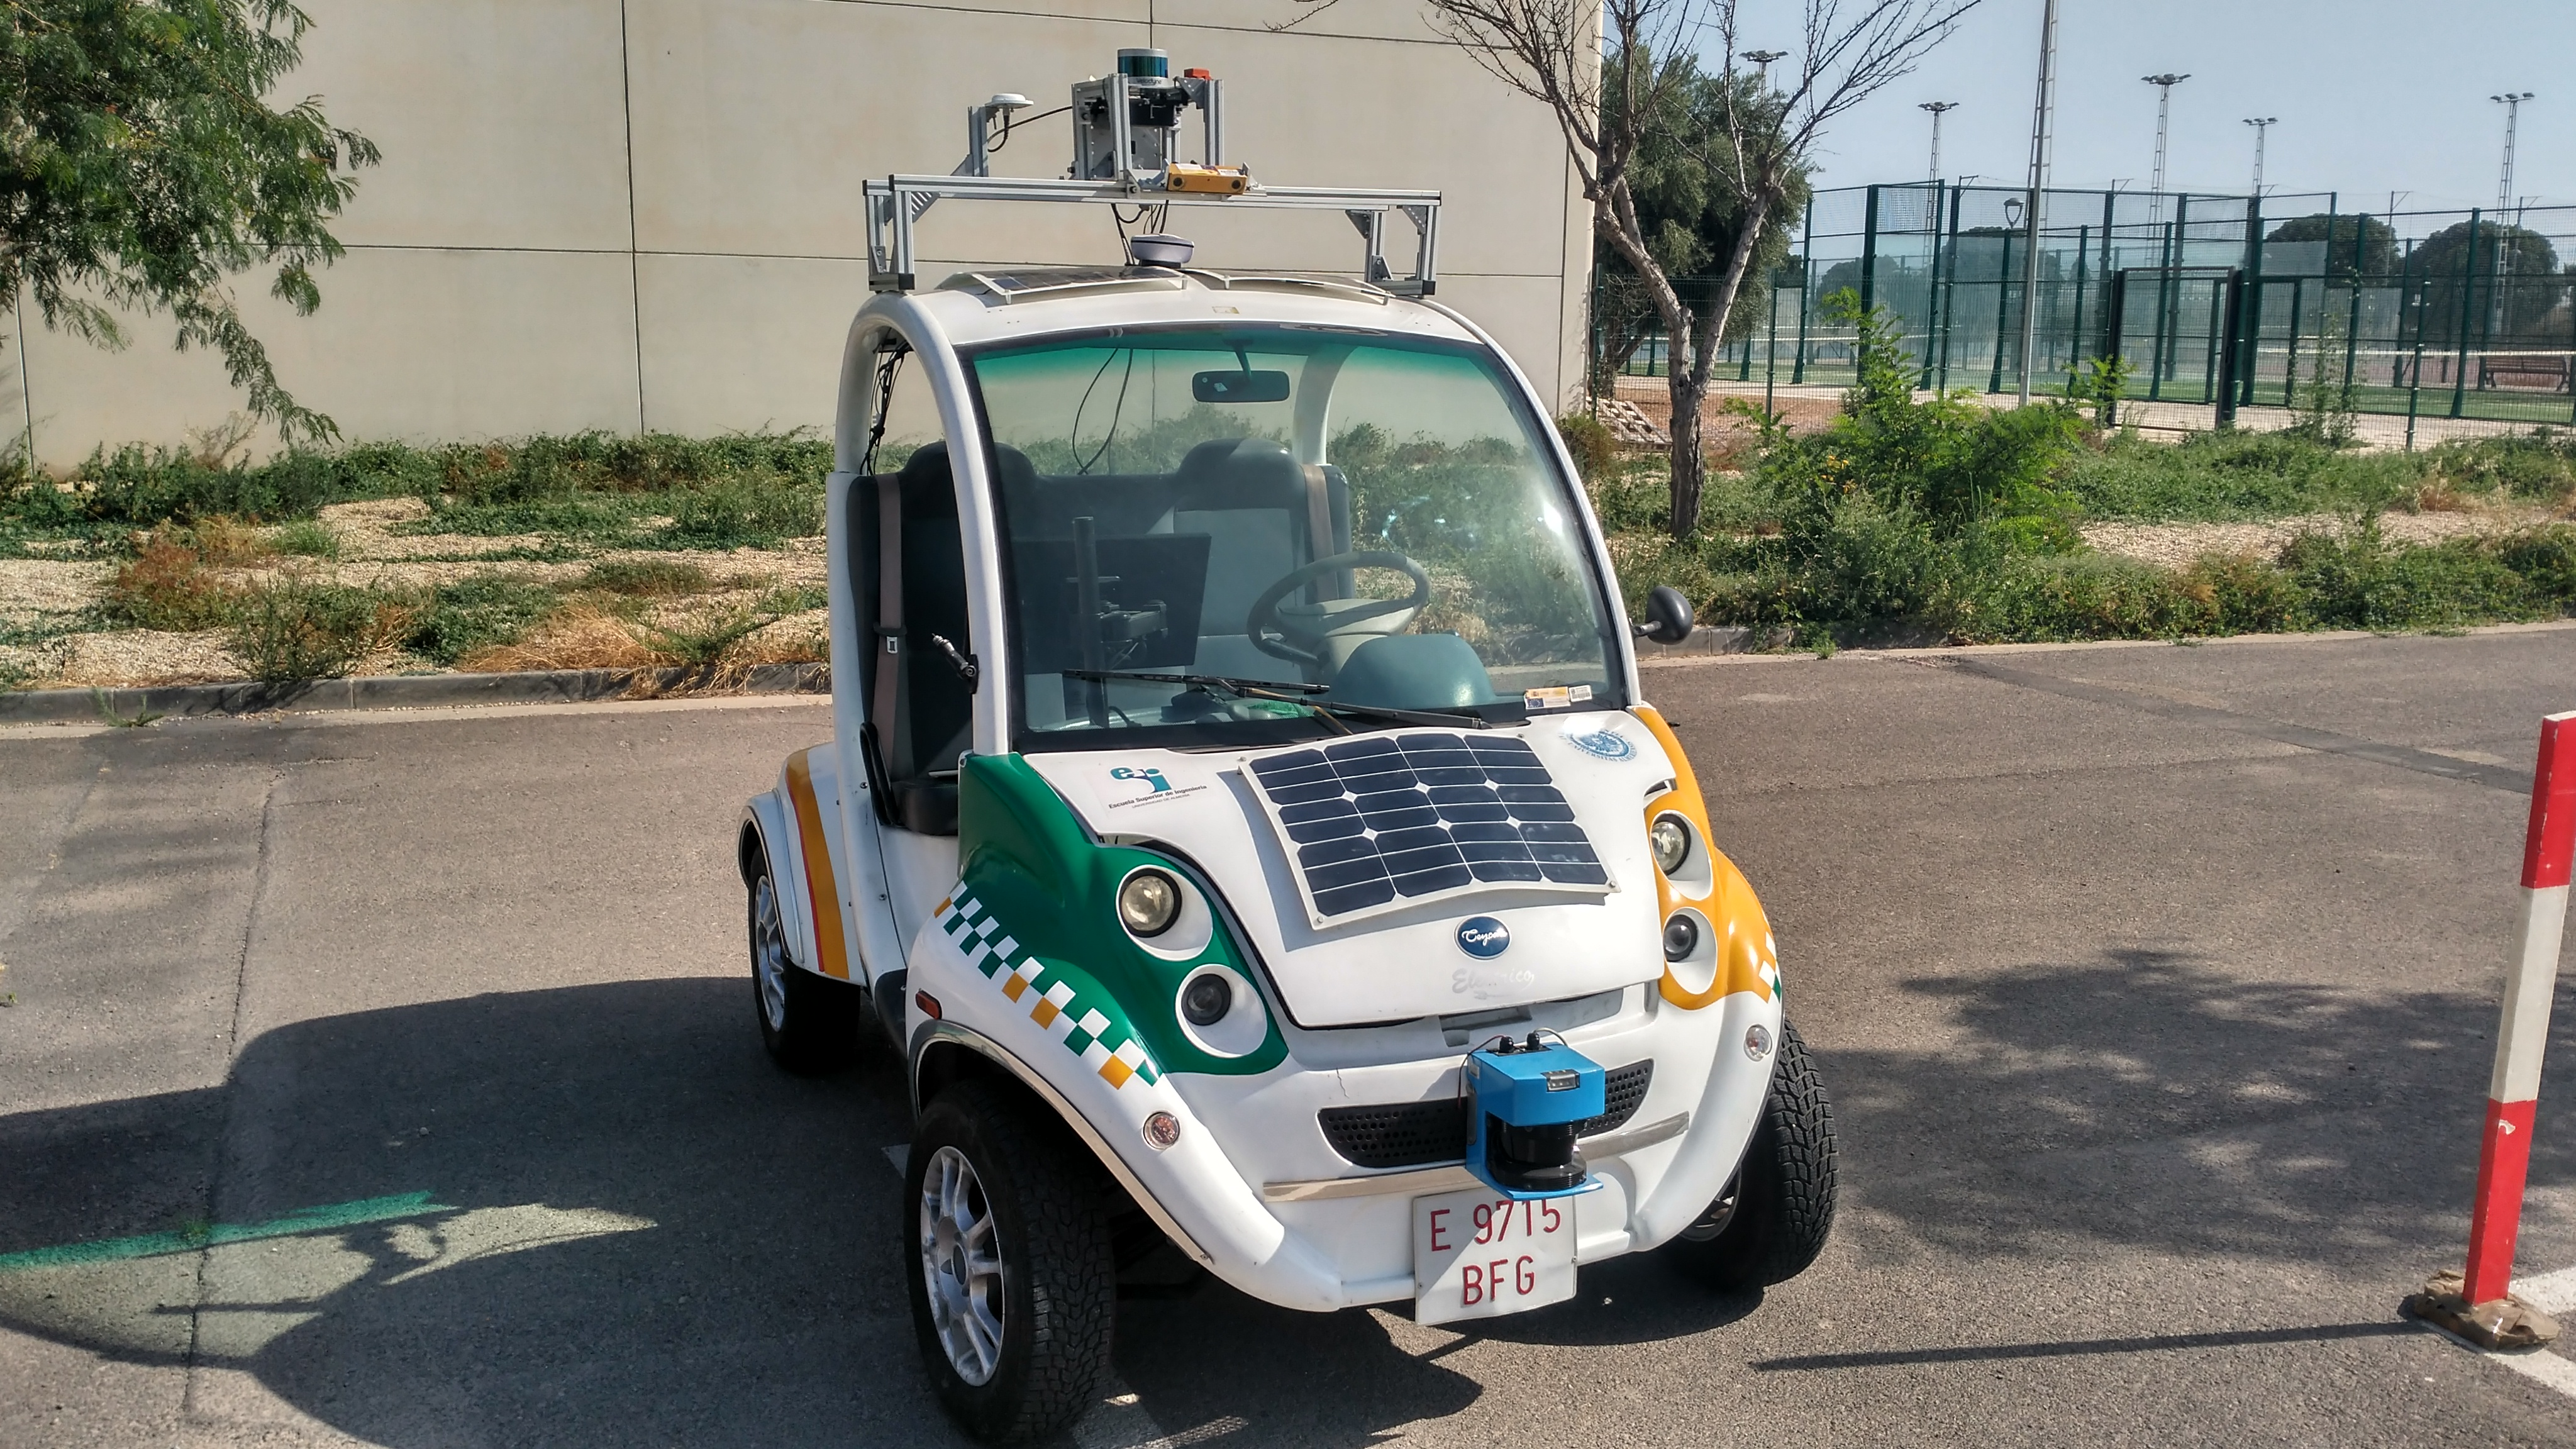
\includegraphics[width=1\textwidth]{Figuras/vehiculo-aparcamientos.jpg}
  \caption{Vehículo UAL-eCARM.}
  \label{fig:vehiculo}
\end{figure}
